\documentclass[12pt]{article}
\usepackage{amsmath}
\usepackage{graphicx}
\usepackage{hyperref}
\usepackage[latin1]{inputenc}
\usepackage{epstopdf} %%package to overcome problem with eps in pdf files

\title{Software Engineering in Practice. My First Open Source Contribution}
\author{Ioannis Petropoulos - t8160107@aueb.gr}
\date{20/05/19}

\begin{document}
\maketitle

% Here is the abstract.
\begin{abstract}
  The most important objective of the Software Engineering in Practice (SEiP) course was to familiarize with the real conditions of open source software development and to encourage the technologies used for this matter. In the meanwhile, that was a unique opportunity to co-operate with engineers that maintain the whole project through a Github repository and be a part of the development team.  
\end{abstract}
%---

\section*{Introduction}
   Open Source software is a trend that is picking up momentum \cite{Forbes} and that is something my university is taking into serious consideration. Personally, SEiP has been a springboard for my academic career. Under the supervision of professor Diomidis Spinellis and the guidence of PhD candidate Antonis Gkortzis, I managed to gather knowledge and gain experience that will make up a solid foundation for my professional evolution in the field of Software Engineering.

\section{Project Understanding}

\paragraph{}
  This should have been the most critical phase of the whole process. Github offers a wide variety of projects to choose from, so you have to choose wisely and be very prudent. But once you do a thorough research, you should find something that fits you perfectly. And that's what happened with me.
  
\paragraph{}
  \textbf{Jarvis by Sukeesh} is an open source project written in Python, inspired by Tony's Stark AI system \cite{Jarvis} and available for Linux, MacOS and Windows. In a few words, Jarvis is a simple personal assistant which works on the terminal and he can do many things such as tell you the weather, find restaurants near you and help you out with many types of calculations.

\paragraph{}
  To be able to understand the project structure, I dedicated a few days testing the features and reading the code and the contribution rules (checked out the PEP 8 guidelines for Python) in order to get familiar with it. In the beggining, chaos prevaled but as I was spending more time with it, it started becoming more clear. After 3 - 4 days, I was able to understand the code structure, so I thought that it's time to get my hands dirty.

\section{Project Contribution}

  To the fun part now, it is time to write code. What I though would be a great idea for Jarvis was to create a plugin that Measures your Body Mass Index and outputs some valuable results.    
  
  \subsection{Change Log}
  
  What I had in mind was an interactive BMI plugin that is easy to use and gives value to the results. Thus, I developed the plugin in Python in about 171 lines of code. Moreover, I refactored the health plugins packaging, due to the fact that they were not easily accessable by the user.
  
  % Use this for pictures
\begin{figure}[tph!]
\centerline{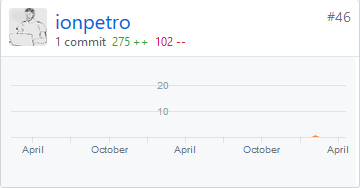
\includegraphics[totalheight=4cm]{contributor.png}}
    \caption{Jarvis contributors list by GitHub}
    \label{fig:verticalcell}
\end{figure}
%-----

  \subsection{Code Quality}
  
  This section will describe how I assured quality to my code.
  
  \subsubsection{Documentation}
  
  Documentation plays an important factor for software development. Every method I used was well documented so in this way, every future contributor would not struggle to understand what my code does. Below you can see an example of a documented method.
  
  \begin{figure}[h]
  \centering
  \begin{minipage}[b]{0.9\textwidth}
    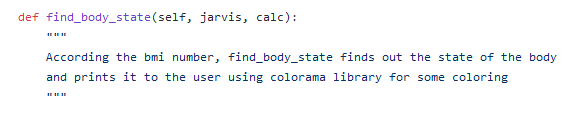
\includegraphics[width=\textwidth]{doc1.png}
    \caption{Flower one.}
  \end{minipage}
  \hfill
  \begin{minipage}[b]{0.9\textwidth}
    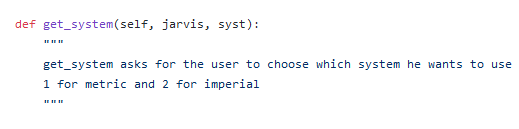
\includegraphics[width=\textwidth]{doc2.png}
    \caption{Flower two.}
  \end{minipage}
\end{figure}
  
  \subsubsection{Linting Errors}
  
 
  
    My final commit to the project was devoted to code quality. Using a Python Library called pylint I did some code analysis on:
    \begin{itemize}
    \item Coding standard (variable names, PEP8 style guide, check imported modules usability)
    \item Error detection
    \item Refactoring duplicated code
    \end{itemize}
    
     \begin{figure}[tph!]
\centerline{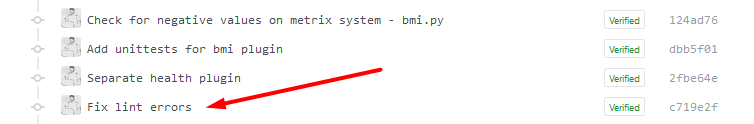
\includegraphics[totalheight=3cm]{lint.png}}
    \caption{Devoted commit on Linting Errors}
    \label{fig:verticalcell}
\end{figure}
%-----
    
    
  \subsection{Continuous Integration}
    
    Jarvis is using Travis CI for Continuous Integration. This part is very important, since the code that you contribute to a project has no meaning and is not going to be accepted if it can not be integrated with the rest of the code. Unfortunately, in the refactoring phase, the plugin of another contributor had some linting errors, so Travis was not able to pass the building phase. However, after contacting the administrator of the project, he undertook the issue and fixed it in one line of code. These things always happen, the important thing is to solve them immediately in communication with the developing team.
      
  \subsection{Testing}
  
    Coding in python, which is a scripting language, you have to write some unit tests in order to test the methods functionality. That's what I did and trust me when I say that the development team was so happy about that. Using the unittest library I wrote 5 different test cases for 2 of my methods.
  
\section{Internal \& External Communication}

    Luckily for me, the development team of Jarvis is very friendly and helpful. Each time I had a difficulty with the code structure, they responded very fast showing me the way through the solution.
 
  \subsection{Development Team integration}
  
    The first time I talked to this guys was through an issue I opened, discussing about a new feature I would like to see to Jarvis in the future.
    
\begin{figure}[tph!]
\centerline{
\includegraphics[totalheight=5cm]{testing.png}}
  \caption{Discussing with DEV team about testing practices}
  \label{fig:verticalcell}
\end{figure}
%-----
  
  \subsection{Presentations}
  
  You can find both of my progress presentations on the GitHub repository: \\
  
  \centerline{
  \textbf{ionpetro/Software-Engineering-in-Practice-Final-Report}
  }
  
  \subsection{GitHub handling}
  
  Withing this course, apart from the coding, we gained valuable knowledge on Version Control Systems such as git. As you can see below, by the time I understood the value of such a tool, I haven't stop using it. Apart from that, I worked on windows-port branch (since I developed the plugin on Windows) and avoided to commit on master branch, which is basically used for production. 
\begin{figure}[h]
\centerline{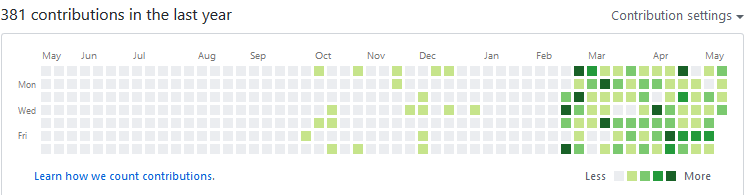
\includegraphics[totalheight=3cm]{gitcommit.png}}
  \caption{Github commits for 2019}
  \label{fig:verticalcell}
\end{figure}
%-----
  
  \subsection{Code Review}
  
  Finally, the administrator of the repository after reviewing my code finally merged the Pull Request to the original repository.
  
  \begin{figure}[h]
\centerline{
\includegraphics[totalheight=3cm]{merged.png}}
  \caption{Merging PR to original repo}
  \label{fig:verticalcell}
\end{figure}
%-----
  
\section{Conclusion}
  
  
\begin{thebibliography}{9}

\bibitem{Forbes} 
Forbes - The trend to open source software and what it means for businesses and consumers.
\\\texttt{https://www.forbes.com/sites/richardfinger/2014/02/04/the-trend
-to-open-source-software-and-what-it-means-for-businesses-and-consumers}.

\bibitem{Jarvis} 
J.A.R.V.I.S | Iron Man Wiki
\\\texttt{https://ironman.fandom.com/wiki/J.A.R.V.I.S.}.

\bibitem{einstein} 
Albert Einstein. 
\textit{Zur Elektrodynamik bewegter K{\"o}rper}. (German) 
[\textit{On the electrodynamics of moving bodies}]. 
Annalen der Physik, 322(10):891–921, 1905.
 
\bibitem{knuthwebsite} 
Knuth: Computers and Typesetting,
\\\texttt{http://www-cs-faculty.stanford.edu/\~{}uno/abcde.html}
\end{thebibliography}
  
\end{document}